\chapter{The $\alpha$-shapes approach to compute the boundaries in target phase space}\label{chap:boundaries_alpha}
The $\alpha$-shape method which is widely used for reconstruction an unknown surface from a set of data points, \cite{guo1997surface}.
We develop a technique based on $\alpha$-shape to obtain an approximation of the boundaries of the set of points obtained from the triangulation refinement.
The aim is to give a criterion to determine the value of the parameter $\alpha$ that gives the better approximation of the boundaries.
The results are given in Section \ref{sec:Tir_alpha} for two different kind of total internal reflection (TIR) collimator.
\section{The $\alpha$-shapes approach}
In this paragraph we give an overview of the state of art about $\alpha$-shapes methods.
Given a finite set $V$ of points $\alpha$-shapes are geometrical objects that give us an approximation of the shape\footnote{It will become clear through this chapter what we intend with the word \textit{shape}.} formed by the points in $V$.\\ \indent
Before giving a formal definition, we explain an intuitive and nice interpretation of $\alpha$-shapes, \cite{lucieer2004alpha}. 
We can think to a mass of a stracciatella ice-cream\footnote{Stracciatella ice cream is made with milk-based ice-cream and fine peaces of chocolate, \cite{Wiki3}.}. If we desire to know the shape formed by the chocolate pieces we can start eating the ice cream using a spoon with a spherical shape and trying to do not remove any piece of chocolate. 
We will obtain a shape formed by arcs and points, see Figure \ref{fig:shape2d} for the two-dimensional case.
\begin{figure}[htbp]\label{fig:shape2d}
\begin{center}
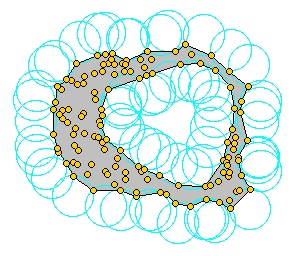
\includegraphics[width=7cm]{shape.jpg}
\label{fig:shape}
\caption{Construction of $\alpha$-shape given a set of points in $\mathbb{R}^2$}
\label{fig:shape2d}
\end{center}
\end{figure}
Straightening the arcs to line segments we obtain broken lines which constitute the boundaries of the so-called $\alpha$-shape formed by the points of the points set $V$. In this example, the chocolates peaces are the points of $V$ and, the parameter $\alpha$ determines the radius of the carving spoon (the spherical spoon in two-dimension is simply a circle). A very small spoon will allow us to eat the entire ice cream without eating any piece of chocolate, while with a huge spoon we are not able to eat any part of the ice cream because we will always take away at least one chocolate peace.\\ \indent 
The previous example might give a better understanding of the definition of $\alpha$-shape first given by Edelsbrunner, Kirkpatrick and Seidel in 1983, \cite{edelsbrunner1983shape}. They describe $\alpha$-shape has a generalization of the convex hull of a finite set of point in the plane. Let be $\alpha$ a not negative number $0\leq\alpha<\infty$. 
If $\alpha$ is equal to $0$ the shape degenerates to the point set $V$. On the other hand, when $\alpha\rightarrow\infty$ the $\alpha$-shape is simply the convex hull of $V$. If $0<\alpha<\infty$ the $\alpha$-shape is a polytope of $V$, \cite{edelsbrunner1994three}. The construction of $\alpha$-shape is closely related to Delaunay triangulation of $V$,\cite{mucke1993shapes}. Therefore, a formal definition of triangulations and Delanauy triangulations is now required. \\ \indent
Given a set $V$ of not all aligned points, let us consider the set $E$ of all the straight line segments whose endpoints are in $V$. 
A triangulation $T$ of $V$ is the maximum subset of $E$ such that all the line segments of $T$ intersect only at their endpoints, \cite{lloyd1977triangulations}. \\ \indent 
The Delaunay triangulation of the points set $V$ has the property (called Delaunay property) that the circle circumscribed by any triangle of $T$ does not contain any point of $V$. A very common used algorithm to construct such triangulation is explained in the following. 
A Delaunay triangulation is constructed by modifying a general triangulation $T$ such that every point satisfies the Delaunay property. 
Therefore, every triangle (or tetrahedron in three dimensions) that does not satisfy such property is flipped such that the new edge is part of the triangulation, see Figure \ref{fig:Delaunay}. 
More precisely, given an arbitrary triangulation $T$ in two-dimension, for each edge $\bar{ab}$ in $T$ which is not on the boundary of the convex hull the two triangles 
$\Delta_{abc}$ and $\Delta_{abd}$ with the common edge $\bar{ab}$ are found. Then, if either the circumcircle of triangle $\Delta_{abc}$ contains point $d$ or the circumcircle of triangle $\Delta_{abd}$ contains point $c$ the edge $\bar{ab}$ cannot be included in the Delaunay triangulation and, therefore, it is flipped such that the other two possible triangles $\Delta_{acd}$ and $\Delta_{bcd}$ are found. The new edge $\bar{cd}$ satisfy the Delaunay property locally and the triangles are added to the Delaunay triangulation.  
\begin{figure}[h]\label{fig:Delaunay}
\begin{center}
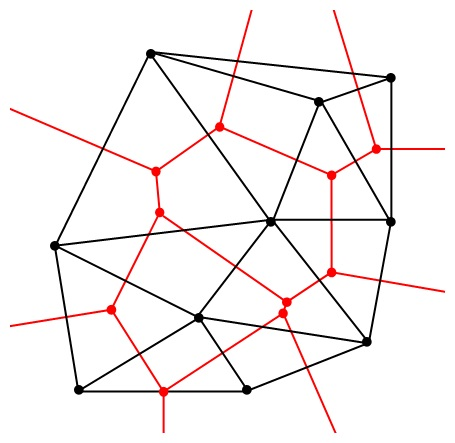
\includegraphics[width=7cm]{Delaunay_Voronoi.jpg}
\label{fig:shape}
\caption{Triangles flipped.}
\label{fig:Delaunay}
\end{center}
\end{figure}
Several others algorithm have been developed to construct a Delaunay triangulation, see for example \cite{lee1980two, renka1997algorithm}.
The Delaunay triangulation $T^\prime$ derived from a triangulation $T$ of a given points set $V$ is unique. It has the property to have the largest minimum angle among all possible triangulation of a point set $V$, \cite{press2007numerical}. 
Delaunay triangulation can be seen as the dual of Voronoi diagram, \cite{fortune1992voronoi}.\\\indent
We give here the definition of Voronoi diagram in two dimensions, (see \cite{brown1979voronoi} for higher dimensions).
In every finite set of point $V = \{v_1, \cdots, v_N\}\subset \mathbb{R}^2$ and for \textit{almost}\footnote{It is needed to specify the word \textit{almost} because some points can have the same distance with two or more points of $V$.} every point $x\in \mathbb{R}^2$, there is a point which is the closest point to $x$. The Voronoi cell of a point $v_\variabile{i}\in V$ contains all points in $\mathbb{R}^2$ which are closer to $v_{\variabile{i}}$, see Figure {fig:Voronoi}. 
The Voronoi diagram is the set of all Voronoi cells, \cite{cazals2005conformal}.
A formal definition of the Voronoi diagram is given in the following.
\begin{defn}
Let $X$ be a metric space with a distance $\textrm{d}$ and $V=\{v_1,\cdots,v_N\}$ a set of point in $X$. The Voronoi cell $V_\variabile{i}$ associated with the point $v_\variabile{i}$ with $v_{\variabile{i}}\in\{1,\cdots,N\}$ is defined as:
\begin{equation}
V_\variabile{i}=\{x\in X\; | \;\textrm{d}(x,v_\variabile{i})\leq \textrm{d}(x,v_\variabile{j}) \quad \forall \variabile{j}\neq \variabile{i} \}\,,
\end{equation}
The Voronoi diagram is defined as the union $U = \bigcup_{\variabile{i}=1}^N V_\variabile{i}$ where $V_{\variabile{i}}\cap V_{\variabile{j}}= \emptyset$ for $\variabile{i}\neq\variabile{j}$.
\end{defn}
Figure \ref{fig:Voronoi}
\begin{figure}[h]\label{fig:Voronoi}
\begin{center}
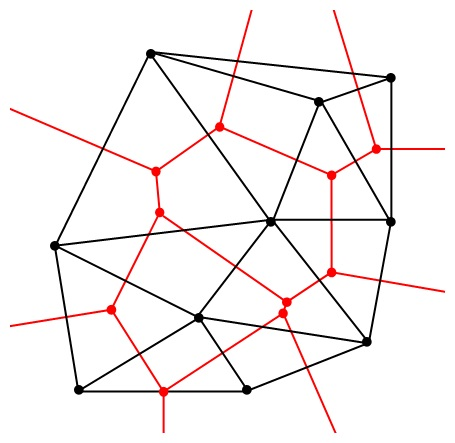
\includegraphics[width=7cm]{Delaunay_Voronoi.jpg}
\caption{The Delaunay triangulation in black is the dual of the Voronoi diagram in red, \cite{Wiki4}.}
\label{fig:Voronoi}
\end{center}
\end{figure}
Delaunay triangulation triangulates the convex hull of $V$ and, therefore it does not constitutes a suitable method for reconstruct the surface formed by a point cloud. 
\\ \indent An important method in surface reconstruction is the $\alpha$-shapes method, \cite{edelsbrunner2010alpha, guo1997surface}. Starting from the Delaunay triangulation $T^\prime$ of a point set $V$, the corresponding $\alpha$-shape of $V$ is formed by the only triangles of $T^\prime$ that satisfy the so-called "$\alpha$-test".
For each triangle we calculate the radius of the circumcircle. If the radius is larger that $\alpha$ the triangle is removed from the shape. The rule of the parameter $\alpha$ is highly significant in this procedure. We would choose $\alpha$ such the better approximation of the shape formed by the points of $V$ is obtained. 
The choice of the parameter $\alpha$ is closely related to the radius of the circumcircles. A possible strategy is to find the radius of the greater empty circumcircle. Thus $\alpha$ is related to the density $\delta$ of the point sets $V$. In particular $\alpha$ is inversely proportional to $\delta$:
\begin{equation}
\alpha=C\frac{1}{\delta}\;,
\end{equation}
with $C$ a constant and $\delta$ is:
\begin{equation}
\delta=\frac{N}{\mbox{surface area}}\; ,
\end{equation}
where $N$ is the number of points in $V$ and the surface area is the area inside the boundaries of the region formed by the points cloud. Hence $\delta$ is given for a fixed point set and the value of $C$ needs to be determined by numerical simulations.\\ \indent 
The $\alpha$-shape procedure can be outlined as follows.
\begin{enumerate}
\item Construct a Delaunay triangulation $T^\prime$ of the point cloud $V$;
\item For every triangles $T^\prime(i)$ calculates the radius $r(i)$ of the circle circumscribed by its vertices;
\item If $r(i)\leq\alpha$ keep the triangle $T^\prime(i)$ in the triangulation;
\item If $r(i)>\alpha$ remove the triangle from the triangulation;
\item For every triangle return the edges (facets in $3$D) referred to only one triangle (tetrahedron in $3$D), the so-called \textit{free boundary} edges.
\end{enumerate}
%% Insert algorithm
%\begin{algorithm}[h]
%\caption{$\alpha$-shape reconstruction}\label{alg:alphashapes}
%\begin{algorithmic}[1]
%\Procedure{$\alpha$-shape}{$V$, $\alpha$}
%\State Construct a Delaunay triangulation of the point cloud $V$
%\State$T^\prime\gets$ all triangles of the Delaunay triangulation
%\State For every 
%\State Calculates the radius of the circle circumscribed by the vertices of every triangle
%\State $r(i) \gets$
%\State For {every triangle in $T^\prime$}
%\State $(\variabile{q}_1^4, \variabile{p}_1^4) \gets \mbox{left and upper corner of source PS: (-\variabile{a}, 1)} $
%\For{$ \variabile{k}= 1 \to 4 $}
%\State Trace the ray with initial coordinates $(\variabile{q}_1^\variabile{k}, \variabile{p}_1^{\variabile{k}})$ in \set{S}{}{};
%\State Calculate the corresponding path $\Pi^{\variabile{k}}$;
%\State $\mbox{Ray}.\variabile{q}\gets [\mbox{Ray}.\variabile{q}, \variabile{q}_1^\variabile{k}]$;
%\State $\mbox{Ray}.\variabile{p}\gets [\mbox{Ray}.\variabile{p}, \variabile{p}_1^\variabile{k}]$;
%\State Store the corresponding path $\Pi^{\variabile{k}}$.
%\State $\mbox{Ray}.\Pi\gets [\mbox{Ray}.\Pi, \Pi^{\variabile{k}}]$;
%\EndFor
%\State VL $\gets [1, 2, 4]$ \Comment{VL = vertices of the left triangle}
%\State VR $\gets [2,3, 4]$   \Comment{VR = vertices of the right triangle}
%\State \Call{Left Triangle}{VL, Ray, $\varepsilon_{\variabile{q}_1}^{\textrm{min}}, \varepsilon_{\variabile{q}_1}^{\textrm{max}}, \varepsilon_{\variabile{p}_1}^{\textrm{min}}, \varepsilon_{\variabile{p}_1}^{\textrm{max}}$}\Comment{Refine the left triangle} 
%\State \Call{Right Triangle}{VR, Ray, $\varepsilon_{\variabile{q}_1}^{\textrm{min}}, \varepsilon_{\variabile{q}_1}^{\textrm{max}}, \varepsilon_{\variabile{p}_1}^{\textrm{min}}, \varepsilon_{\variabile{p}_1}^{\textrm{max}}$} \Comment{Refine the right triangle} \\
%\Return ;
%\EndProcedure
%\end{algorithmic}
%\end{algorithm}
%\\
%Let us define a Voronoi diagram in a metric space.
%The simplest case that we can have is the two-dimensional case that is the case where $X=\mathbb{R}^2$.
%The tuple $\mathcal{S}=\{1,\cdots,n\}\subset \mathbb{R}^2$ is now a set of points. The Voronoi diagram of $\mathcal{S}$ is a subsection of $\mathbb{R}^2$ such that every other region around a point $p\in \mathcal{S}$ contains all points that are closer to $p$ than to every point in $\mathcal{S}$. A triangulation of the point set $\mathcal{S}$ is a set of edges $\mathcal{E}$ whose extremes are points of $\mathcal{S}$ such that the faces of each triangle are bounded by three edges and any edge that is not in $\mathcal{E}$ intersects one of the existing edges. The Delaunay triangulation is the dual graph of the Voronoi diagram: it consists of vertices (the points in $\mathcal{S}$) and it has an edge between two vertices if the two corresponding faces share an edge. \\
\indent $\alpha$-shapes are a powerful tool to reconstruct surfaces. However, there exist surfaces that are not described well by $ \alpha $-shapes. Indeed for some surfaces there exist no value of $\alpha$ that includes all desired triangles and deletes all undesired triangles. For example, it can be difficult to obtain a good approximation of a shape formed by a non-uniform points set if the parameter $\alpha$ is determined according to the density of the point cloud. Furthermore, the $\alpha$-shape method does not work well when the shape has a sharp turn or a joint. In this case $\alpha$-shapes often give a "webbed-foot" appearance at such joints since they improperly connect the adjacent surfaces. To overcome this issue, Teichmann and Capps presented an alternative approach to establish the value of $\alpha$, \cite{teichmann1998surface}. Their density-scaled $\alpha$-shapes method constitutes an improvement of "classical" $\alpha$-shapes.
% BRIDGE
%There are several ways to determine the value of $\alpha$ \cite{mandal1997selection}; we provide a technique that exploits the conservation of the \'{e}tendue in phase space. The essence of our approach is explained in the following.

%The first step of this method is to make a triangulation of the point cloud.
%Then the key idea is to compute somehow the point-density of each point and use this to get an approximation of the point density of a triangle. In this way one can reduce the $\alpha$-value in areas where the triangle's point density (see equation \ref{delta_t} for the definition) is higher than average in such a way that is possible to obtain a finer level of detail for areas that have an higher density.
%More precisely, each point $ \textbf{p}\in \mathcal{S} $ has a local point density defined as
%\begin{equation}
%\delta (\textbf{p})= \sum_{\textbf{q}\in \mathcal{S}}\Big( 1-\frac{\textrm{d}(q,p)}{\lambda}\Big) \qquad \forall \textbf{q} \mbox{\;\;such that\;\;} \textrm{d}(\textbf{p},\textbf{q})<\lambda\,,
%\end{equation}
%where $ \lambda $ is the constant radius of the local neighborhood and $\textrm{d}(\textbf{x},\textbf{y})$ is the Euclidean distance.
%When local density is larger than the average, that is when
%\begin{equation}
%\delta (\textbf{p}) >\frac{1}{| \mathcal{S} |}\sum_{\textbf{q}\in \mathcal{S}}\delta (\textbf{q})
%\end{equation}
%we know some properties about the region surrounding $\textbf{p}$.
%For instance, if the point set is uniformly distributed then it is possible to find areas with a high-density in the case where there are two closely separated surfaces.  In point sets of non-uniform distribution, high densities are found when the surface presents a joint discontinuity. The algorithm developed by Teichmann and Capps is structured as follow.
%After computing density information for each point they make a triangulation of the point set. Then they calculate the average density  $\delta(t)$ for each triangle $\Delta_{abc}$ defined as:
%\begin{equation}
%\delta(t)=\frac{\delta(a)+\delta(b)+\delta(c)}{3 \mu}\,,
%\label{delta_t}
%\end{equation}
%where $\mu$ is the global average density of the entire point set $\mathcal{S}$.
%If $\delta(t)$ is greater than $1$ the density of the point cloud is higher. Hence is necessary to define another value of $\alpha$:
%\begin{equation}
%\alpha^{\;\prime} = \frac{\alpha}{\delta(t)^\sigma}
%\end{equation} where $\sigma$ is a value that is adjusted by the user.
%If  $\delta$ is less than $1$ the $\alpha$-value is not modified.
%In this way it is possible to have a finer precision on the shape formed by the point set where the density is higher than the average density. Hence it is possible to distinguish two separated objects with different density.

% We want to determine the boundaries in phase space
% Jorg
% It is useful to understand whether the approximation is correct
\section{Determination of $\alpha$ using \'{e}tendue conservation} \label{sec:Tir_alpha}
As mentioned in Section \ref{sec:PSconcept} \'{e}tendue can be seen as an area in a two-dimensional phase space. 
Therefore, given an optical system with a line segment source $\point{S} = [-\variabile{a}, \variabile{a}]$, the \'{e}tendue at the source coincides with the area of the entire PS \set{S}{}{}, given by:
\begin{equation}\label{eq:etenduesource}
U = 4\n_1 \variabile{a} \sin(\myangle_1^{\textrm{max}})\,,
\end{equation}
 where $\variabile{a}$ is the half length of the source, $\n_1$ the index of refraction of the medium in which the \point{S} is located and $\myangle_1^{\textrm{max}}$ is the maximum value of the angle that the rays make with the normal $\boldsymbol{\nu}_1$ of the source.\\ \indent 
For some optical systems, all the rays emitted by the source arrive to the target, for some others there are also rays that can end up to other detectors. 
The \'{e}tendue of a set of rays is defined by the area they occupy in PS. Indicating with \set{R}{$1$}{}$(\Pi)$ the regions in source PS formed by the rays that reach the target and with \set{R}{}{} the corresponding regions at the target, the \'{e}tendue $U_1$ at source of the rays that reach the target is:
\begin{equation}\label{eq:etenduesumsource}
U_1 = \sum_\Pi{U_1\big(\mbox{\set{R}{$1$}{}}(\Pi)\big)},
\end{equation}
where the sum is over all possible paths $\Pi$ and $U_1\big(\mbox{\set{R}{$1$}{}}(\Pi)\big)$ is the contribution to \'{e}tendue given by the rays inside the region 
\set{R}{$1$}{}$(\Pi)$ in source PS given by:
\begin{equation}\label{eq:etendueintegralsource}
U_1\big(\mbox{\set{R}{$1$}{}}(\Pi)\big) = {\int\!\!\int}_{\emph{R}_1(\Pi)} \textrm{d}\variabile{q}\,\textrm{d}\variabile{p}.
\end{equation}
Similarly the \'{e}tendue at the target of the rays emitted by the source is:
\begin{equation}
U_\textrm{t}= \sum_\Pi{U_\textrm{t}\big(\mbox{\set{R}{}{}}(\Pi)\big)},
\end{equation}
with
\begin{equation}\label{eq:etendueintegraltarget}
U_\textrm{t}\big(\mbox{\set{R}{}{}}(\Pi)\big) = {\int\!\!\int}_{\emph{R}(\Pi)} \textrm{d}\variabile{q}\,\textrm{d}\variabile{p}.
\end{equation}
In order to determine the value of $\alpha$ in the $\alpha$-shape procedure that better approximates the boundaries $\partial$\set{R}{}{}$(\Pi)$ we use \'{e}tendue conservation, i.e. $U_{\textrm{t}}= U_1$ as explianed in the following.\\ \indent
The $\alpha$-shapes method is applied to every region \set{R}{}{}$(\Pi)$ for a range of values of $\alpha$;
   for each value an approximation of the boundaries $\partial$\set{R}{}{}$(\Pi)$ is obtained and
   the intersection points $\variabile{q}^{\textrm{\,max}}(\Pi,\variabile{p})$ and $\variabile{q}^{\textrm{\,min}}(\Pi,\variabile{p})$ between $\partial$\set{R}{}{}$(\Pi)$
and the horizontal lines $\variabile{p}=const$, with $\variabile{p}\in[-1,1]$, are computed for every path $\Pi$.
Therefore Equation (\ref{eq:etendueintegraltarget}) becomes
\begin{equation}\label{eq:etenduetarg}
 U_\textrm{t}\big(\mbox{\set{R}{}{}}(\Pi)\big)= \int_{-1}^{1}{\Big(\variabile{q}^{\textrm{\,max}}(\Pi,\variabile{p})-\variabile{q}^{\textrm{\,min}}(\Pi,\variabile{p})\Big)} \textrm{d}\variabile{q}\,\textrm{d}\variabile{p}.
\end{equation} In case more than two intersection points between line $\variabile{p}=const$ and $\partial$\set{R}{}{}$(\Pi)$ occur, the previous equation needs to be generalized. Suppose that $\variabile{r}$ intersection points $\big(\variabile{q}^{\,\variabile{i}}(\Pi,\variabile{p}), \variabile{p}\big)_{\variabile{i} = 1, \cdots, \variabile{r}}$ are found. 
First their $\variabile{q}$ coordinates are ordered in ascending order, second the target \'{e}tendue is calculated using
\begin{equation}\label{eq:etenduetarg1}
 U_\textrm{t}\big(\mbox{\set{R}{}{}}(\Pi)\big) =\sum_{\variabile{i} = 1}^{\variabile{m}} \int_{-1}^{1}
{(\variabile{q}^{\,2\variabile{i}}(\Pi,\variabile{p})}-{\variabile{q}^{\,2\variabile{i}-1} (\Pi, \variabile{p}) )} \textrm{d}\variabile{q}\,\textrm{d}\variabile{p}\,,
\end{equation}
where $\variabile{m}$ is the integer part of $\variabile{r}/2$ with $\variabile{r}$. 
The integrals in Equation (\ref{eq:etenduetarg}) and (\ref{eq:etenduetarg1}) are calculated discretizing the interval $[-1, 1]$
   into $\nbin=100$ sub-intervals of equal length, the so-called bins, and using the trapezoidal rule to approximate the integral.
   Note that by increasing the value of $\alpha$, the area inside the $\alpha$-shape increases and, consequently, the \'{e}tendue raises.
\\ \indent Eventually, matching the value of the \'{e}tendue at the source $U_1$ with the value of the \'{e}tendue at the target $U_{\textrm{t}}$, a unique value $\alpha_{c}$ of $\alpha$  is determined. Implemented the $\alpha$-shapes procedure with $\alpha = \alpha_c$, the best approximation of the boundaries $\partial$\set{R}{}{}$(\Pi)$ is found and the intensity at the target can be calculated.\\ \indent If two intersection points between $\variabile{p}=const$ and $\partial$\set{R}{}{}$(\Pi)$ are found the target intensity is calculated using Equation ($\ref{eta2}$), otherwise the generalized equation:
\begin{equation}
I_{PS}(\variabile{p}) = \sum_{\Pi, \variabile{i} }\int_{\variabile{q}^{\,2\variabile{i}-1}(\Pi, \variabile{p})}^{\variabile{q}^{\,2\variabile{i}}( \Pi, \variabile{p})}L(\variabile{q}, \variabile{p})\textrm{d}\variabile{q}\,,
\label{eq:Ips}
\end{equation}
where the summation over $\Pi$ is for all the paths $\Pi$ for which the intersection $\variabile{p} = const$ and \set{R}{}{}$(\Pi)$ is not empty, and the summation over $\variabile{i}$ is for all $\variabile{i} = 1,2, \cdots, \variabile{m}$.
In order to clarify our idea we apply the method to a simple optical system.
\\ \indent Let us consider the two-faceted cup introduced in Chapter \ref{chap:raytracing} and depicted in Figure \ref{fig:cup}. The half length of the source is $\variabile{a}=2$, the maximum angle is $\myangle_1^{\textrm{max}} = \pi/2$ and \point{S} is located in air, i.e. $\n_1=1$. Therefore, the total \'{e}tendue is $U=8$. For the two-faceted cup all the rays emitted by \point{S} arrive to \point{T}, hence from \'{e}tendue conservation we obtain that $U_{\textrm{t}} =U_1 = 8$.
For some optical systems, not all the rays emitted by the source arrive to the target.  
% Explain the idea: use etendue conservation
% Do the example for the two faceted cup
% Explain the TIR collimator
\section{Results for a TIR collimator}
We apply ray tracing in PS for two different kinds of total internal reflection (TIR)-collimators to compute the target intensity. 
In this paragraph we use the $\alpha$-shapes approach to calculate the boundaries of the regions with positive luminance. Let us describe the TIR-collimator depicted in Figure \ref{fig:tir}. It is an optical system symmetric with respect to the $z$-axis, it consists of a lens (central curve), two broken lines adjacent to the lens,
two curved lines on each side and a top formed by a horizontal segment. The lens (line $2$) and the broken lines, formed by a collection of three segments (lines $3, 4, \mbox{ and } 5$ and $9, 10 \mbox{ and } 11$), are refractive line segments while the curved lines (labeled with $6$ and $8$) are designed in such a way that light is internally reflected (which explains the name TIR).
The light source $\mathcal{S}$ (line $1$) and the target $\mathcal{T}$ (line $12$) are two straight line segments normal to the optical axis.
The source $\point{S}= [-2,2]$ is located at a height $\variabile{z}_{1} = 0.3$ from the $\variabile{x}$-axis.
 The target $\point{T}= [-9.7, 9.7]$ is parallel to the source and is located at a height $ \variabile{z}= 8.2$ and both are located inside air ($\n_1=1$).
The volume inside the collimator is filled with a material with index of refraction $\n_2=1.5$ (e.g. glass).
The collimator is surrounded by two vertical lines (lines $13$ and $15$) and two horizontal lines ($12$ and $14$) that receive the light exiting from the optical system; among these the horizontal one at the top is assumed to be the light target, and it is located at a small distance from the top (line $7$). 
\begin{figure}[h]
  \begin{center}
  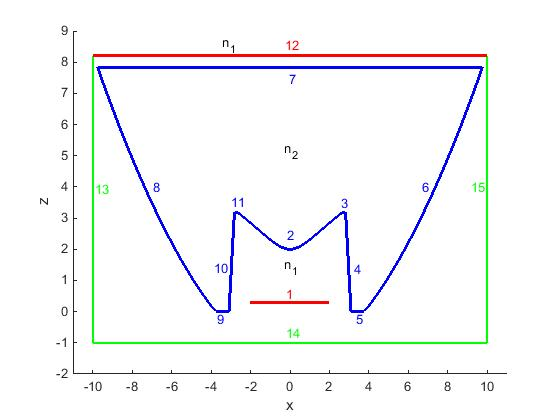
\includegraphics[width=7.7cm]{TIR.jpg}
  \end{center}
  \caption{Shape of the TIR-collimator. Each surface of the system is labeled with a number.
   The shape of the collimator is shown with a blue line.
   Three detectors depicted with green lines (surfaces $13$, $14$, and $15$) are located at the left, the right and the bottom of the optical system.
The sagitta of the lens is approximately $1.17$}
  \label{fig:tir}
\end{figure}
Using PS ray tracing explained in Section \ref{sec:PS_raytracing} with around $1.9 \cdot 10^4$ rays traced, seven different paths are found. In Figure \ref{fig:sourcePS} the distribution of the rays traced at the source PS \set{S}{}{} is shown, where we depicted with the same color the rays that follow the same path. Seven different paths are found. The yellow rays follow the path $\Pi_1 = (1, 2, 7, 12)$;
   the red rays follow the path $\Pi_2 ~= ~(1, 10, 8, 7, 12)$; the green rays follow the path $\Pi_3 = (1, 4, 6, 7, 12)$;
   the blue rays follow the path $\Pi_4= (1, 11, 7, 12)$ and the magenta rays follow the path $\Pi_5= (1, 3, 7, 12)$. The rays located inside the white areas correspond to rays that do not reach the target, they follow either path $\Pi_6 = (1, 10, 7, 8, 13)$ or path $\Pi_7 = (1,4,7,6,15)$ and they do not give any contribution to the target intensity.
\begin{figure}[h]
  \begin{center}
  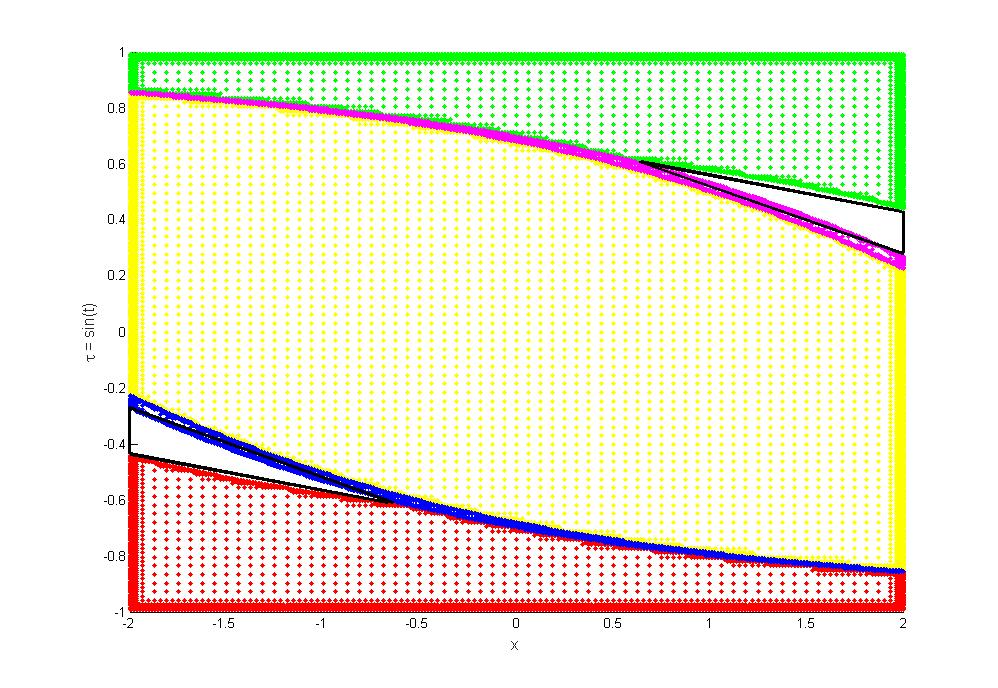
\includegraphics[width=7.7cm]{source1.jpg}
  \end{center}
  \caption{Distribution of the rays on source phase space. Around $1.9 \cdot 10^4$ rays are traced using the triangulation refinement with parameters:
  $\varepsilon_\variabile{q}^\textrm{min} = 0.1 ,$ $ \varepsilon_{\variabile{p}}^\textrm{min} = 5\cdot 10^{-2}, $ $\varepsilon_{\variabile{q}}^\textrm{max} = 9\cdot 10^{-3}, \varepsilon_\variabile{p}^\textrm{max} = 4.5 \cdot 10^{-3}$. Rays that belong to the same region are depicted with the same color. The rays located inside the white areas do not reach the target. The boundaries of the two white regions are approximated by triangles depicted with black lines.}
  \label{fig:sourcePS}
\end{figure}
Note that, given two adjacent paths the regions $\mbox{\set{R}{$1$}{}}(\Pi)$ in \set{S}{}{} have usually a common boundary. 
Since for this system not all the rays emitted by the source arrive to the target, the target \'{e}tendue $U_{\textrm{t}}$ needs to be compared with the \'{e}tendue $U_1$ at the source given by only those rays that reach the target (the rays that follow paths $\Pi_6=(1,10,8,7,12)$ and 
$\Pi_7 = (1,4,7,6,15)$ are discarded). To this purpose $U_1$ is calculated by removing from the total area $U$ of \set{S}{}{} those areas occupied by the regions formed by the rays that hit the left and the right detector (white regions in Figure $\ref{fig:tir}$).  For the TIR colllimator in Figure \ref{fig:tir} $U = 8$. Hence, $U_1$ can be approximated by:
 \begin{equation}
 U_{1}\approx 8-2A_{T}
 \end{equation}
 where $A_{T}$ is the approximated area of each of the white regions in Figure $\ref{fig:tir}$ that is the area of the triangles shown in Fig. \ref{fig:sourcePS} with black lines. Then, $U_{\textrm{t}}$ is calculated several times from Equation (\ref{eq:etenduetarg}) where every time the boundaries $\partial$\set{R}{}{}$(\Pi)$ are obtained by using $\alpha$-shapes for a different value of $\alpha$. The better approximation of $\partial$\set{R}{}{}$(\Pi)$ gives the closer value of $U_{\textrm{t}}$ to the exact \'{e}tendue. 
Matching $U_1$ with all the approximation of $U_{\textrm{t}}$ we find the best value $\alpha_c$ of $\alpha$ that approximates $\partial$\set{R}{}{}$(\Pi)$ and, therefore $U_{\textrm{t}}$. Figure \ref{fig:etendueTS} shows that a value of $\alpha_c = 0.041$ is obtained for a set of $1.9\cdot 10^4$ rays.
 \begin{figure}[h]
  \begin{center}
  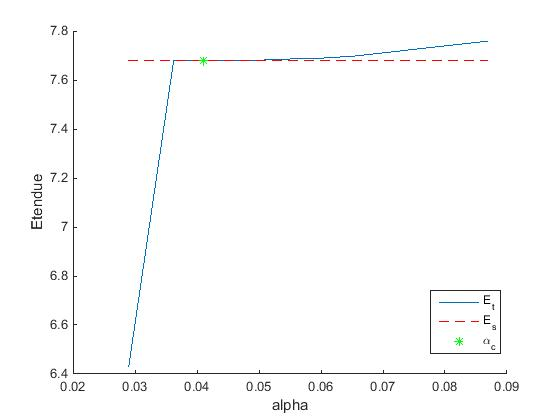
\includegraphics[width=7.7cm]{etendue.jpg}
  \end{center}
  \caption{\footnotesize{The source and the target \'{e}tendue are depicted with the dotted red line and the blue line, respectively.
  $U_\textrm{t}$ is computed for a range of values for $\alpha$. $U_1 \approx 7.68$
   The green dot indicates the value of $\alpha_c = 0.041$ which gives the best approximation of the boundaries $\partial$\set{R}{}{}$(\Pi)$ at the target.
   Around $1.9 \cdot 10^4$ rays have been traced in PS.
  }}
  \label{fig:etendueTS}
\end{figure}
Applying $\alpha$-shapes with $\alpha=\alpha_c$, a good approximation of $\partial$\set{R}{}{}$(\Pi)$ is found. In Fugure \ref{fig:targetPS} we show the boundaries 
$\partial$\set{R}{}{}$(\Pi)$ in target PS \set{T}{}{} with $\alpha_c=0.041$ and tracing $1.9*10^4$ rays.
  \begin{figure}[h]
  \begin{center}
  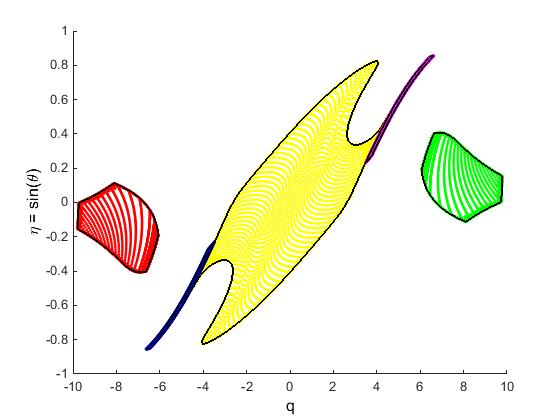
\includegraphics[width=7.7cm]{target.jpg}
  \end{center}
  \caption{\footnotesize{Target phase space representation of a set of $1.9 \cdot 10^4$ rays.
  Rays that follow the same path are depicted with the same color. The choice of the colors for each path is the same as in Figure $\ref{fig:sourcePS}$. The boundaries $\partial$\set{R}{}{}$\Pi$ are computed through the $\alpha$-shapes method with $\alpha = \alpha_c = 0.041$.}}
  \label{fig:targetPS}
\end{figure}
Once the boundaries are computed, the target intensity $I_{PS}(\variabile{p})$ for every $\variabile{p}\in[-1,1]$ is given by Equation (\ref{eta2}). 
To validate our method we compare the $PS$ intensity with the $MC$ intensity. 
To this purpose a partitioning $P_2:-1=\variabile{p}_{0}<\variabile{p}_1<\cdots<\variabile{p}_{\nbin}=1$ of the interval $[-1,1]$ into $\nbin=100$ bins is considered. 
The averaged and normalized PS intensity $\hat{I}_{PS}$ is calculated for every 
$\big(\variabile{p}^{\variabile{h}+1/2} = \frac{1}{2}(\variabile{p}^{\variabile{h}+1}, \variabile{p}^{\variabile{h}})\big)_{\variabile{h}=0, \cdots, \nbin-1}$ dividing the PS averaged intensity by the total \'{e}tendue:
\begin{equation}\label{eq:normalized_PS_intensity}
\hat{I}_{PS}(\variabile{p}^{\variabile{h}+1/2}) = \frac{1}{U_{\textrm{t}}}\int_{\variabile{p}_{\variabile{h}}}^{\variabile{p}_{\variabile{h}+1}} I_{PS}(\variabile{p})\textrm{d}\variabile{p}
\end{equation}
The averaged and normalized MC intensity $\big(\hat{I}_{MC}(\variabile{p}^{\variabile{h}+1/2})\big)_{\variabile{h} = 0, \cdots, \nbin-1}$ intensity is given by
\begin{equation}\label{eq:normalized_MC_intensity}
\hat{I}_{MC}(\variabile{p}^{\variabile{h}+1/2}) = \frac{}{}
\end{equation} 
% In Figure \ref{fig:intensity_TIR} we show the PS intensity and the MC intensity with
Finally, defining the error between the approximates intensity $\hat{I}_{A} (A = PS, MC)$ and the reference intensity $\hat{I}_{ref}$:
%\begin{equation}\label{eq:error}
%\mbox{error} = \frac{\sum_{\variabile{h}= 1}^{\nbin}| \hat{I}_{A}(\variabile{p}^{\variabile{h}}) - \hat{I}_{\mbox{ref}}(\varaibile{p}^{\variabile{h}})|}{\nbin}
%\end{equation}
In Figure \ref{fig:error_nr_tir} we show how the error decreases increasing the number of rays traced for both PS ray tracing and MC ray tracing.
The MC and PS intensities are calculated several times increasing the number of rays to improve the accuracy.
Both the approximate intensities are compared with an intensity taken as a reference.
For some optical systems, there is an explicit solution for the target intensity but this is not the case of the TIR-collimator.
Therefore, a MC simulation with $1,7 \cdot 10^8$ rays is run to obtain the normalized intensity $\hat{I}_{\mbox{ref}}$ which is used as reference.
We show how the error,
defined as:
\begin{equation}\label{error}
\mbox{error} = \frac{\sum_{h = 1}^{Nb}| \hat{I}_{PS}(\eta_h) - \hat{I}_{\mbox{ref}}(\eta_h)|}{Nb}\,,
\end{equation}
%and is computed for both the PS and MC intensities.
decreases for increasing number of rays.
%As a result, the error gradually decreases.
Table \ref{tab:table} describes how the number of rays traced affects the error and shows the correlation between $\alpha_c$ and the number of rays, which is
determined by the values of $\epsilon_{x_{min}}$, $\epsilon_{\tau_{min}}$, $\epsilon_{x_{max}}$ and $\epsilon_{\tau_{max}}$ as explained in Section \ref{sec:method}\ref{subsec:triangulation1}. The values of $\alpha_c$ are selected according to the method
presented in Section \ref{sec:method}$\ref{sec:alpha}$.
 Then, the intensity for the MC method, $\hat{I}_{MC}$, is computed.
Replacing $\hat{I}_{PS}$ with $\hat{I}_{MC}$ in Equation (\ref{error}), the error between the reference intensity and the intensity computed with the MC method is
calculated.
Increasing the number of rays traced in MC ray tracing, the error gradually decreases.
In Table $\ref{tab:table2}$ the numerical results found are reported.
\begin{table}[htbp] \label{tab:table}
\centering
\caption{\bf Error values of the PS intensity}
\begin{tabular}{lllllll}
 \hline  Number \\ of rays\;  & $\epsilon_{x_{min}} $  & $\epsilon_{x_{max}} $   \;     & $\epsilon_{\tau_{min}}$\;
  & $\epsilon_{\tau_{max}}$\; & $\alpha_c$  & error \\
  \hline 
 $3\,363$ & $0.9$  & $0.1$  & $0.50$  & $0.025$ & $0.119$ & $1.20\cdot10^{-3}$ \\
$6\,949$  & $0.5$  & $0.050$  & $0.25$  & $0.020$ & $0.098$ & $2.50\cdot 10^{-4}$  \\
$15\,870$  & $0.4$  & $0.025$  & $0.02$  & $0.001$ & $0.050$ & $5.49\cdot 10^{-4}$ \\
 $37\,455$  & $0.2$  & $0.020$  & $0.10$ & $0.005$ & $0.037$ & $2.00\cdot 10^{-5}$ \\
 $66\,855$ & $0.1$  & $0.009$  & $0.05$  & $0.004$ & $0.020$ & $1.00\cdot 10^{-5}$ \\
 \hline
 \end{tabular}
 \label{tab:table}
 \end{table}
\begin{table}[htbp]
\centering
\caption{\bf Error values of the MC intensity}
\begin{tabular}{ll} \hline   Number of rays\; & $\mbox{error}_{MC}$\\ \hline $972$  & $2.10\cdot10^{-3}$ \\
$9\,714$  & $6.69\cdot 10^{-4}$  \\ $97\,103$  & $2.08\cdot 10^{-4}$ \\ $971\,627$  & $7.00\cdot 10^{-5}$ \\ $9\,716\,519$  & $2.00\cdot 10^{-5}$ \\
 \hline
 \end{tabular}
 \label{tab:table2}
 \end{table}
\noindent In Figure $\ref{fig:error}$, the results listed in Table $\ref{tab:table}$ and Table $\ref{tab:table2}$ are shown where the red line depicts the behavior of the error for the PS
intensity, and the blue line indicates the error for the MC simulation.
\begin{figure}[h!]
  \begin{center}
  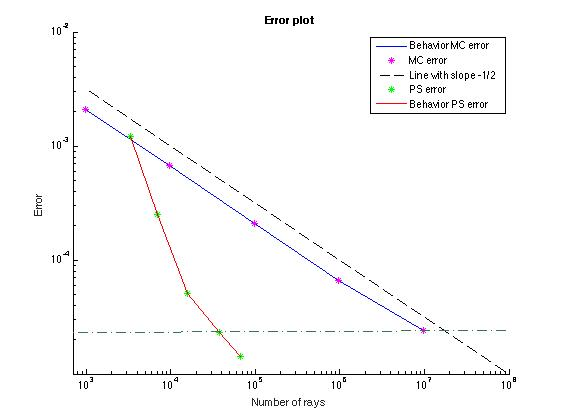
\includegraphics[width=7.7cm]{error.jpg}
  \end{center}
  \caption{\footnotesize{ The red line depicts the error between the intensity on phase space and the exact intensity.
 The blue line shows the error between the Monte Carlo intensity and the exact intensity.
  The dashed line represents a straight line with the slope equal to $-\frac{1}{2}$.
  The horizontal dotted line shows that an error equal to $2.00 \cdot  10^{-5}$ can be obtained tracing at least $10^2$ times fewer rays in phase space.}}
  \label{fig:error}
\end{figure}
\noindent The intensity profile $\hat{I}_{PS}
$ obtained with the phase space method and tracing $66\,855$ rays is depicted in Fig. \ref{fig:intensityMCPS} with a red line.
$\hat{I}_{PS}$ is hardly distinguishable from $\hat{I}_{\mbox{ref}}$ (dashed and blue line in Figure $\ref{fig:intensityMCPS}$).
Figure $\ref{fig:error}$ shows that an error equal to $2.00 \cdot  10^{-5}$ can be obtained by tracing around $9.7 \cdot 10^{6}$ for
Monte Carlo while in phase space only around $3.7 \cdot 10^4$ rays need  to be traced to obtain the same accuracy of the intensity.
  \begin{figure}[h]
    \centering
    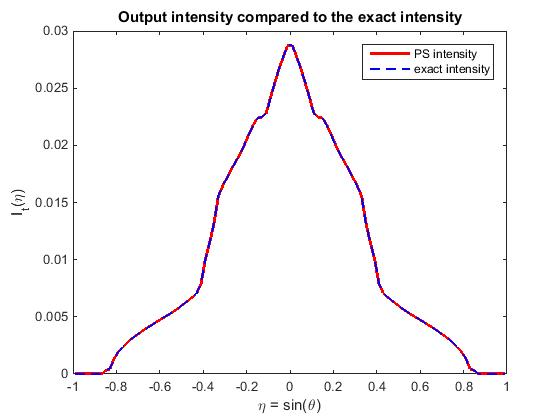
\includegraphics[width=\textwidth]{intensity.jpg}
\caption{\footnotesize{The red line shows the PS intensity at the target of the TIR-collimator. The exact intensity is depicted with the dotted blue line.
The exact intensity is computed using the MC method for a set of $15$ millions of rays. For the PS intensity a set of $6.6\cdot 10^4$
rays is considered and $\alpha_c = 0.02$ is chosen to compute the boundaries $\partial R_{\textrm{t}, \Pi_j}$. The approximate intensity can hardly be distinguished from the exact
intensity. }}
  \label{fig:intensityMCPS}
\end{figure}
 

%Since the PS intensity depends on $\variabile{p}=\n_1\sin(\myangle)\in[-1,1]$ instead of $\optangle\in[-\pi/2, \pi/2]$,
% Intensity
% MC intensity
% Error

% Second TIR collimator
% Show the results 








































